\documentclass[handout,12pt]{beamer}
\usepackage[utf8]{inputenc}
\usetheme{Singapore}

\usepackage{minted}
\setminted[Javascript]{fontsize=\small, tabsize=2, breaklines, linenos}

\usepackage{tabularx}
\usepackage{upquote}


\title{Introduction to JavaScript}
\subtitle{For web browsers}
\author{Julius Putra Tanu Setiaji}
\date{NUS Hackers Hackerschool, 2018}

\begin{document}
	\frame{\titlepage}
	
	\section{Introduction}
	\subsection{}
	\begin{frame}
		\frametitle{NUS Hackers}
		\begin{center}
			

\includegraphics[width=0.5\linewidth]{NUSHackers}

\url{http://nushackers.org}
\end{center}

\begin{center}
	\textbf{Hacker}school
	
	Friday \textbf{Hacks}
	
	\textbf{Hack} \& Roll
	
	NUS \textbf{Hacker}space
\end{center}

	\end{frame}
	
	\begin{frame}
		\frametitle{About Me}
		Hi! I'm Julius. My GitHub is \url{https://github.com/indocomsoft}\\
				
		A Year 1 Computer Science Undergraduate who loves hacking and building systems.\\
			
		I took CS1101S taught in JavaScript and have been doing web development intensively for the past 2 years.\\
		
		(Not so important) I also enjoy Aerospace Engineering, Music Theory and History {\tiny (my favourite games are KSP and EU4 hit me up if you play those too)}
	\end{frame}
	
	\begin{frame}
		\frametitle{Table of Contents}
		\tableofcontents
	\end{frame}
	
	
	\begin{frame}
		\frametitle{Required Software}
		\begin{itemize}
			\item \textbf{Google Chrome} (\url{http://chrome.google.com/})
			\item \textbf{Sublime Text 3} (\url{http://www.sublimetext.com/3}) or any decent text editor
		\end{itemize}
		
		\textbf{Materials} can be found at \url{https://drive.google.com/drive/folders/1gaiBcnkGRwZ3w3z1j8H_CZqpV6iPcQmz?usp=sharing}
		
		\textbf{Code snippets} at \url{https://hackmd.io/0bxMdu7SSOijPO089-G75w?view}
	\end{frame}
	
	\begin{frame}
		\frametitle{JavaScript Drum Kit}
		\begin{itemize}
			\item A sneak peek on what we will be building today.
			\item Do raise your hands if you're lost!
		\end{itemize}
	\end{frame}

	\begin{frame}
		\frametitle{Why and What is Javascript?}
		\begin{itemize}
			\item HTML \& CSS defines a webpage's structure and style statically.
			\item JavaScript allows more dynamic aspect of the web:
			\begin{itemize}
				\item User interaction
				\item Modifying the webpage
				\item Communicating with a server
			\end{itemize}
			\item Javascript is:
			\begin{itemize}
				\item dynamic and weakly-typed
				\item multi-paradigm (prototype-based object-oriented, imperative, functional, event-driven)
			\end{itemize}
		\end{itemize}
	\end{frame}
	
	\begin{frame}
		\frametitle{Short History}
		\begin{itemize}
			\item It was first included by Netscape Navigator in 1995.
			\item It has since been standardised by Ecma Int'l.
			\item Consequently, the standard is called ECMAScript.
			\item There are several editions of the standard:
			\begin{itemize}
				\item ECMAScript 5.1
				\item ECMAScript 6 (ES6, also called ES2015)
				\item ECMAScript 7 (ES7, also called ES2016)
			\end{itemize}
			\item For the purpose of today's Hackerschool, we will focus more on ES6.
		\end{itemize}
	\end{frame}
	
	\begin{frame}
		\frametitle{Resources}
		\begin{itemize}
			\item Mozilla Developer Network (\url{https://developer.mozilla.org/en-US/docs/Web/JavaScript}) offers one of the best documentation of JavaScript.
			\item Even Microsoft is redirecting its web docs to MDN\footnotemark
		\end{itemize}
		\footnotetext[1]{\url{https://blogs.windows.com/msedgedev/2017/10/18/documenting-web-together-mdn-web-docs/}}
	\end{frame}
	
	\begin{frame}
		\frametitle{Following along}
		\begin{itemize}
			\item All modern web browsers have an integrated JavaScript interpreter. You can run codes in this presentation by using the console.
			\item For Firefox and Chrome, go to \alert{Developer Tools} (keyboard shortcut: Ctrl+Shift+I or Command + Option + I)
		\end{itemize}
	\end{frame}
	
\section{Primitive Data Types}
\subsection{}
\begin{frame}[fragile]
	\frametitle{Data Types}
	There are 6 primitive data types in ES6:
	\begin{itemize}
		\item Null
		\item Undefined
		\item \textbf{Number}
		\item \textbf{String}
		\item Symbol
		\item \textbf{Boolean}
	\end{itemize}
\end{frame}

\begin{frame}[fragile]
	\frametitle{3 Important Primitive Data Types}
	\begin{itemize}
		\item \textbf{Number} = A numeric data type in the double-precision 64-bit floating point format
		\begin{minted}{Javascript}
typeof 1101			// returns "number"
typeof 5.00			// returns "number"
typeof Math.PI	// returns "number"
		\end{minted}
		\item \textbf{String} = sequence of characters
		\begin{minted}{Javascript}
typeof "asd"		// returns "string"
typeof 'asd'		// returns "string"
		\end{minted}
		\item \textbf{Boolean} = only 2 possible values: \texttt{true} and \texttt{false}
		\begin{minted}{Javascript}
typeof true		// returns "boolean"
typeof false	// returns "boolean"
		\end{minted}
	\end{itemize}
\end{frame}

\section{Variable, Data Structures, Flow Control}
\subsection{}
\begin{frame}[fragile]
	\frametitle{Variable Declaration}
	\begin{itemize}
		\item Traditionally, variables are declared using \texttt{var}.
		\item However, since ES6, there are 2 more ways to declare variable, \texttt{let} (allows reassignment) and \texttt{const} (prevents reassignment).
		\item The difference is in scoping\footnotemark. Generally, I would advise using \texttt{let} and \texttt{const}.
		\footnotetext{\texttt{var} is function-scoped while \texttt{let} and \texttt{const} are block-scoped}
		\begin{minted}{Javascript}
var name = "Julius"
let mood = "happy"
const birthyear = 1997
name = "indocomsoft" // OK
mood = "excited"		 // OK
birthyear = 2001		 // Error
		\end{minted}
	\end{itemize}
\end{frame}

\begin{frame}[fragile]
	\frametitle{Array}
	\begin{itemize}
		\item \textbf{Array} is an ordered collection of data.
		\begin{minted}{Javascript}
// Empty array
[]						

let arr = [1, 2, 3, "a", true]
a[0] // 1
a[3] // "a"
a[4] // true
		\end{minted}
		\item There are many built-in Array methods. Look them up at MDN!
	\end{itemize}
\end{frame}

\begin{frame}[fragile]
	\frametitle{Object}
	\begin{itemize}
		\item \textbf{Object} is a data structure containing data and instructions (fields and methods).
		\begin{minted}{Javascript}
// Empty object
{}
														
// Literal object
let car = { "brand": "Tesla", "model": "X", "production_year": 2015 } 
car["brand"]						// "Tesla"
car.model								// "X"
car["production_year"]	// 2015
car.production_year			// 2015
car.name								// undefined
		\end{minted}
	\end{itemize}
\end{frame}

\begin{frame}[fragile]
	\frametitle{Function}
	\begin{itemize}
		\item \textbf{Function} is a code snippet.
		\begin{minted}{Javascript}
function plusOne(x) {
	return x + 1;
}
plusOne(2)                  // Returns 3

let plusOne = (x) => x + 1; // Arrow functions
plusOne(2)                  // Returns 3

// Functions can be passed around
let op = (f, v) => f(v);
op(plusOne, 5);             // Returns 6
		\end{minted}
	\end{itemize}
\end{frame}

\begin{frame}[fragile]
	\frametitle{if - else if - else Flow Control}
	\begin{itemize}
		\item Logical operators: \texttt{\&\&} (and), \texttt{||} (or), \texttt{!} (not)\pause
		\item Comparison operators: \texttt{==} (equality), \texttt{!=} (inequality), \texttt{===} (identity/strict equality), \texttt{!==} (non-identity/strict inequality), \texttt{>}, \texttt{>=}, \texttt{<}, \texttt{<=}.\pause
		\begin{minted}{Javascript}
let x = 10;
if (x < 10) {
	console.log("smaller")
} else if (x > 10) {
	console.log("larger")
} else {
	console.log("equal")
}
		\end{minted}
	\end{itemize}
\end{frame}

\begin{frame}[fragile]
	\frametitle{Truthy and Falsy}
	\begin{itemize}
		\item Values that translate to \texttt{true} and \texttt{false} respectively.
		\item List of falsy values:
		\begin{minted}{Javascript}
if (false)
if (null)
if (undefined)
if (0)
if (NaN)
if ('')
if ("")
		\end{minted}
		\item Other values are by definition truthy
		\begin{minted}{Javascript}
let me = { "name": "Julius", "age": 21 }
if (me.address) console.log("address exists!")
else console.log("address is missing")
		\end{minted}
	\end{itemize}
\end{frame}

\begin{frame}
	\frametitle{JavaScript is dynamic and weakly typed!}
	\begin{itemize}
		\item Be careful! JavaScript was designed to not throw error as far as it could. So, given an ambiguous instruction, it will try to guess what you really meant.
		\item A case in point: WAT \url{https://www.destroyallsoftware.com/talks/wat}
	\end{itemize}
\end{frame}


\section{HTML DOM}
\subsection{}
\begin{frame}
	\frametitle{Brief Review on HTML \& CSS}
	\begin{itemize}
		\item HTML defines a document's structure
		\item CSS defines a document's style
	\end{itemize}
\end{frame}

\begin{frame}
	\frametitle{The HTML DOM}
	\begin{itemize}
		\item HTML DOM (Document Object Model) is the Web API that allows JavaScript to dynamically change a webpage.
		\item In JavaScript, the API can be accessed using the \mintinline{Javascript}{document} object.
		\item A HTML Document can be represented as a tree:
\begin{center}
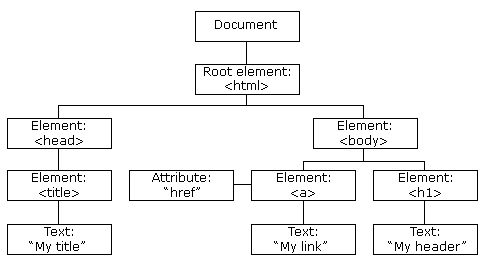
\includegraphics[width=0.7\linewidth]{HTML-DOM}
\end{center}

	\end{itemize}
\end{frame}

\subsection{Selecting an element}
\begin{frame}
	\frametitle{Selecting an element}
	\begin{itemize}
		\item Use the \mintinline{Javascript}{document.querySelector}\footnotemark function.
		\begin{center}
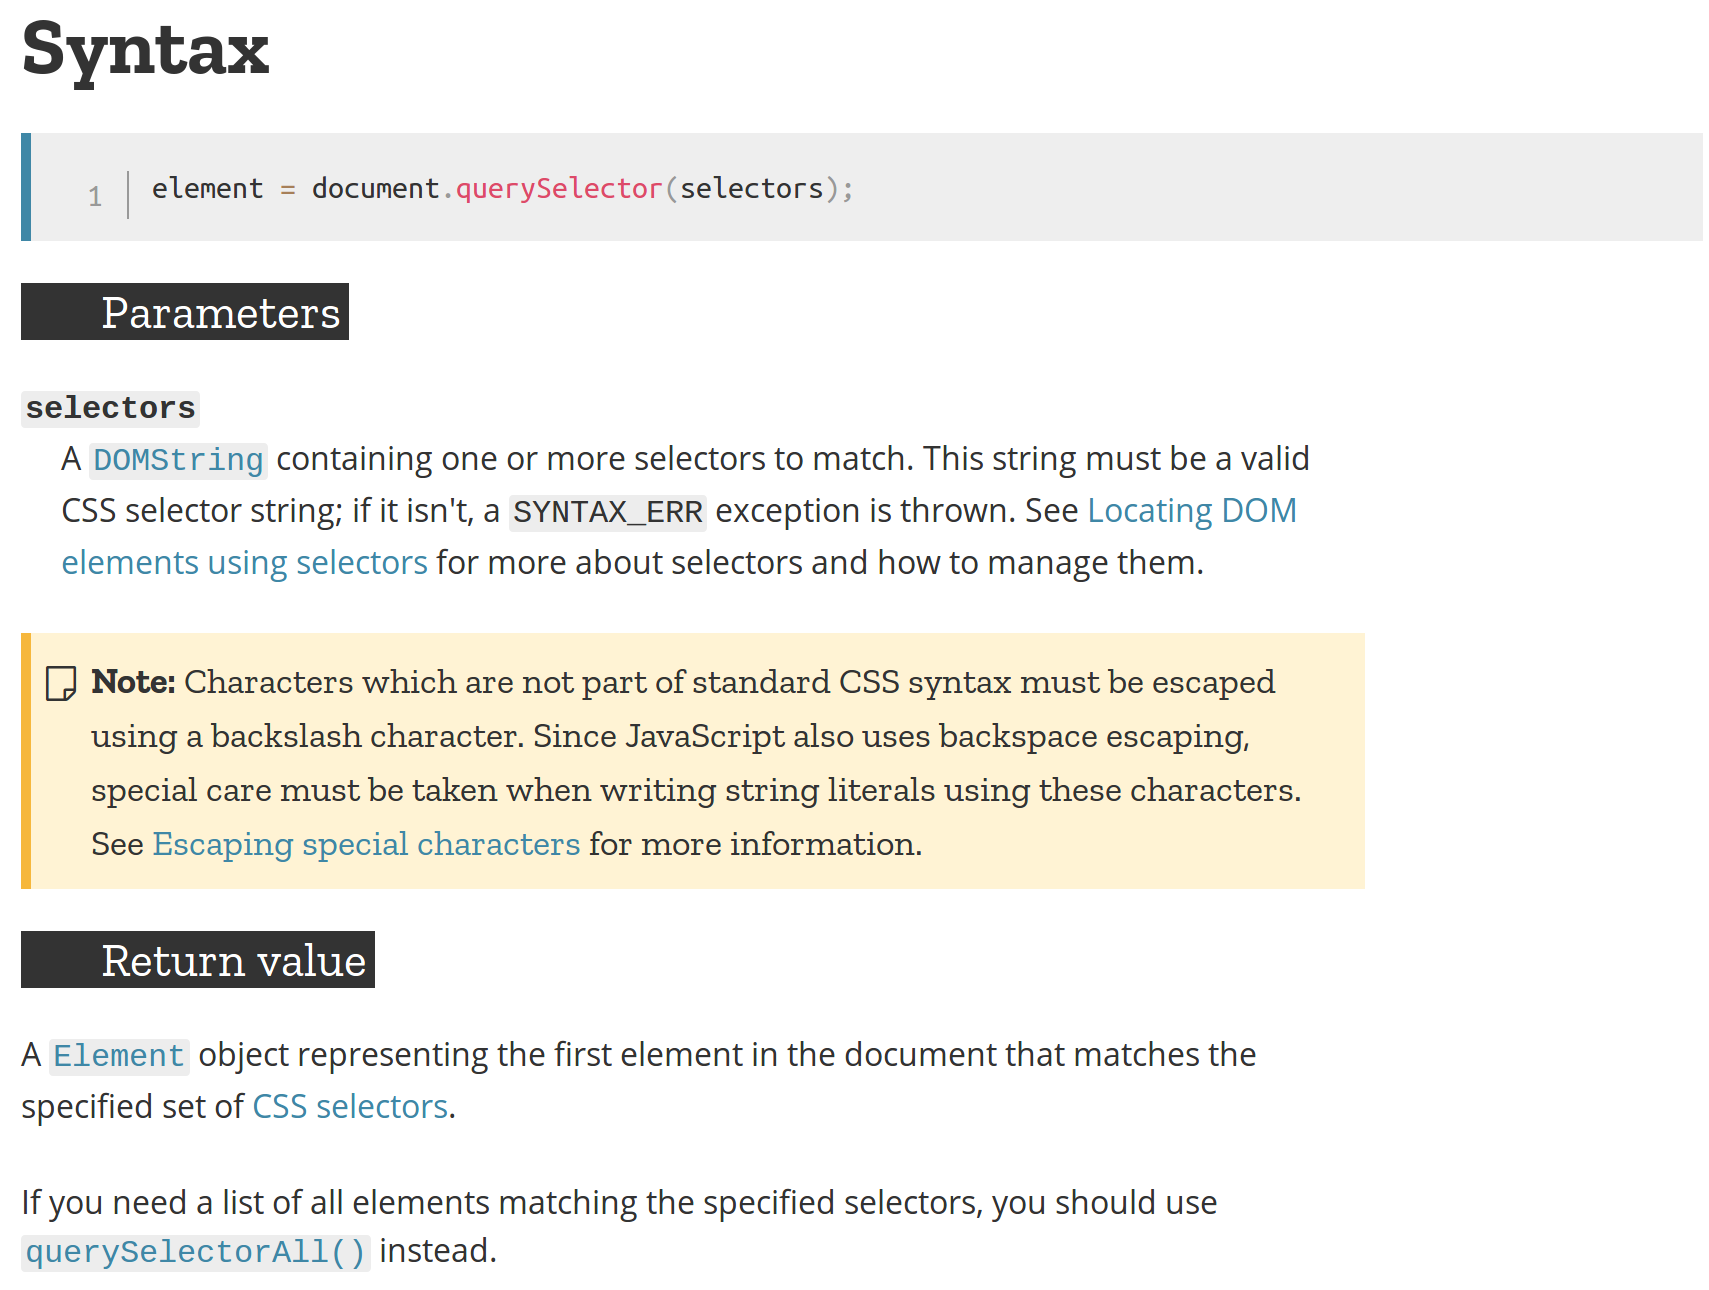
\includegraphics[width=0.7\linewidth]{querySelector-MDN}
\end{center}
	\end{itemize}
	\footnotetext[3]{\url{https://developer.mozilla.org/en-US/docs/Web/API/Document/querySelector}}
\end{frame}

\begin{frame}[fragile]
	\frametitle{Example of \mintinline{Javascript}{document.querySelector}}
		\begin{minted}{Javascript}
document.querySelector("audio[data-key='65']");
		\end{minted}
What does this do?		
	\begin{itemize}
		\item \mintinline{Javascript}{document.querySelector} will select the first element.
		\item CSS selector string \mintinline{Javascript}{"audio[data-key='65']"}
		\begin{itemize}
			\item an element with an audio tag
			\item whose data-key attribute is 65
		\end{itemize} 
	\end{itemize}
\end{frame}

\begin{frame}[fragile]
	\frametitle{The \mintinline{HTML}{<audio>} tag and \mintinline{HTML}{data-*} attribute}
	\begin{minted}{HTML}
<audio data-key="65" src="sounds/clap.wav"></audio>
	\end{minted}
	\begin{itemize}
		\item The \mintinline{HTML}{<audio>} tag is used to embed sound content in documents, containing one or more audio sources specified in the \texttt{src} attribute or with a \mintinline{HTML}{<source>} elements.
		\item \texttt{data-*} attribute is a new feature introduced in HTML5. It is for extensibility purposes, allowing us to store extra information on standard HTML elements.
	\end{itemize}
\end{frame}

\subsection{Playing audio file}
\begin{frame}[fragile]
	\frametitle{Playing audio file}
	\begin{itemize}
		\item An \mintinline{HTML}{<audio>} element provides a method to play the audio it contains: \mintinline{Javascript}{audioElement.play();}
		\item Thus, to play audio, we can do this:
		\begin{minted}{Javascript}
let clap = document.querySelector("audio[data-key='65']");
clap.play();
let hihat = document.querySelector("audio[data-key='83']");
hihat.play();
let kick = document.querySelector("audio[data-key='68']");
kick.play();
// So on and so forth
		\end{minted}
	\end{itemize}
\end{frame}

\begin{frame}[fragile]
	\frametitle{DRY! (Don't Repeat Yourself)}
	\begin{itemize}
		\item Remember your CS1010/CS1101S! Abstraction!
		\begin{minted}{Javascript}
function playSound(keyCode) {
	let audio = document.querySelector("audio[data-key='" + keyCode + "']");
	audio.play();
}

playSound(65);
		\end{minted}
		\pause
		\item Now try running \mintinline{Javascript}{playSound(65);} in rapid succession. The same audio waits until it is finished before playing again!
	\end{itemize}
\end{frame}
\begin{frame}[fragile]
	\frametitle{Starting audio before the previous play finishes}
	\begin{itemize}
		\item How do you solve this? Use the HTML DOM, \mintinline{Javascript}{HTMLMediaElement.currentTime}\footnotemark!
	\end{itemize}
	\begin{minted}{Javascript}
function playSound(keyCode){
	let audio = document.querySelector("audio[data-key='" + keyCode + "']");
	audio.currentTime = 0; // Add this
	audio.play();
}

playSound(65);
playSound(65);
	\end{minted}
	\footnotetext[4]{\url{https://developer.mozilla.org/en-US/docs/Web/API/HTMLMediaElement/currentTime}}
\end{frame}

\subsection{Adding/Removing a CSS class}
\begin{frame}[fragile]
	\frametitle{CSS class}
	\begin{itemize}
		\item Recall how we apply styles to HTML documents: by including a CSS stylesheet, and then adding appropriate class attributes to the HTML elements.
		\item For example, each key in the drum kit has class \texttt{key}
		\begin{minted}{HTML}
<div data-key="65" class="key">
	<kbd>A</kbd>
	<span class="sound">clap</span>
</div>
		\end{minted}
		\begin{minted}{CSS}
.key { /* various styles */ }
.playing {
	transform: scale(1.1);
	border-color: #ffc600;
	box-shadow: 0 0 1rem #ffc600;
}
		\end{minted}
	\end{itemize}
\end{frame}

\begin{frame}[fragile]
	\frametitle{Adding/Removing a CSS class}
	\begin{itemize}
		\item Now, what we want to do is to add a CSS class \texttt{playing} when the audio is playing, and then remove the class when the key has been scaled up.
		\item This can easily achieved through a HTML DOM method \mintinline{Javascript}{Element.classList}\footnotemark
		\begin{minted}{Javascript}
		let clapKey = document.querySelector("div[data-key='65']");
		clapKey.classList.add('playing');
		clapKey.classList.remove('playing');
		\end{minted}
	\end{itemize}
	
	\footnotetext[5]{\url{https://developer.mozilla.org/en-US/docs/Web/API/Element/classList}}
\end{frame}

\subsection{Events and Listeners}
\begin{frame}[fragile]
	\frametitle{Events and Listeners}
	\begin{itemize}
		\item As mentioned in slide 4, JavaScript is event-driven.
		\item Analogy:
		\begin{tabularx}{\linewidth}{|X|X|}
			\hline
			\textbf{(Events)} & \textbf{(Listeners)} \\
			\textbf{When the customers requests for...}		&  \textbf{Inform these people...} \\ \hline
			Spaghetti		& Chef \\ \hline
			Washroom		& Toilet manager \\ \hline
			Pizza				& Pizza Hut, Canadian Pizza, Domino's \\ \hline
		\end{tabularx}
		\item \textbf{Event}: signal from the browser that something has happened. The browser then conveys this signal to all \textbf{listeners} of that event.
	\end{itemize}
\end{frame}
\begin{frame}[fragile]
	\frametitle{Callback functions as Listener}
	\begin{itemize}
		\item In JavaScript, we have callback functions as listeners that is invoked whenever an event occurs.
		\item To register a function as a listener, we use the HTML DOM function \mintinline{Javascript}{document.addEventListener(eventType, callback)}\footnotemark
			\begin{minted}{Javascript}
document.addEventListener('keydown', () => {
	console.log(event);
});
			\end{minted}
		\item \mintinline{Javascript}{console.log()} is the equivalent of print in other languages.
	\end{itemize}
	\footnotetext[6]{\url{https://developer.mozilla.org/en-US/docs/Web/API/EventTarget/addEventListener}}
\end{frame}

\section{Putting everything together}
\subsection{}
\begin{frame}
	\frametitle{Putting everything together}
	When user hits the key:
	\begin{enumerate}
		\item Play the sound associated with the key
		\item At keypress, add \texttt{.playing} class to the \mintinline{HTML}{<div>} associated with the key
		\item When it has been completely scaled, remove \texttt{.playing} class from \mintinline{HTML}{<div>}
	\end{enumerate}
\end{frame}

\begin{frame}[fragile]
	\frametitle{{Play the sound associated with the key}}
	\begin{minted}{Javascript}
function playSound(keyCode){
	let audio = document.querySelector("audio[data-key='" + keyCode + "']");
	audio.currentTime = 0;
	audio.play();
}
	\end{minted}
\end{frame}

\begin{frame}[fragile]
	\frametitle{At keypress, add \texttt{.playing} class}
	\begin{minted}{Javascript}
function playSound(keyCode) {
	let audio = document.querySelector("audio[data-key='" + keyCode + "']");
	let key = document.querySelector("div[data-key='" + keyCode + "']");
	key.classList.add('playing');
	audio.currentTime = 0;
	audio.play();
}
\end{minted}
\end{frame}

\begin{frame}[fragile]
	\frametitle{Filter for Bad Input}
	\begin{itemize}
		\item \texttt{data-key} is represents the ASCII code of the keys.
		\item If the key pressed is not any of the keys in the HTML document, then do nothing.
	\end{itemize}
		\begin{minted}{Javascript}
function playSound(keyCode) {
	let audio = document.querySelector("audio[data-key='" + keyCode + "']");
	let key = document.querySelector("div[data-key='" + keyCode + "']");
	if (audio !== null) {
		key.classList.add('playing');
		audio.currentTime = 0;
		audio.play();
	}
}
		\end{minted}
\end{frame}

\begin{frame}[fragile]
	\frametitle{Add keydown listener}
	\begin{itemize}
		\item Change parameter to be \mintinline{Javascript}{event}, and \mintinline{Javascript}{keyCode} to be \mintinline{Javascript}{event.keyCode} and register \mintinline{Javascript}{playSound} as a listener.
	\end{itemize}
	\begin{minted}{Javascript}
function playSound(event) {
	let audio = document.querySelector("audio[data-key='" + event.keyCode + "']");
	let key = document.querySelector("div[data-key='" + event.keyCode + "']");
	if (audio !== null) {
		key.classList.add('playing');
		audio.currentTime = 0;
		audio.play();
	}
}
document.addEventListener('keydown', playSound);
	\end{minted}
\end{frame}

\begin{frame}[fragile]
	\frametitle{Listeners on multiple elements}
	\begin{itemize}
		\item We can do so using \mintinline{Javascript}{document.querySelectorAll}\footnotemark and \mintinline{Javascript}{Array.forEach}\footnotemark\pause
		\begin{minted}{Javascript}
let keys = document.querySelectorAll('.key');
keys.forEach(key => key.addEventListener('transitionend', event => { event.target.classList.remove('playing'); }));
		\end{minted}
	\end{itemize}
	\footnotetext[6]{\url{https://developer.mozilla.org/en-US/docs/Web/API/Document/querySelectorAll}}
	\footnotetext[7]{\url{https://developer.mozilla.org/en-US/docs/Web/JavaScript/Reference/Global_Objects/Array/forEach}}
\end{frame}

\begin{frame}
	\frametitle{Talk to us!}
	\begin{itemize}
		\item \textbf{Feedback form}: \url{https://tinyurl.com/HS2018JS}
		\item \textbf{Upcoming hackerschool}:\\
		Introduction to Machine Learning Part 1
	\end{itemize}
\end{frame}

\end{document}